\chapter{QUERY}

Karena data-data peta pada MapInfo selain berbentuk data spasial, adapula data yang berbentuk atribut seperti misal kolom d\_nop pada tabel layer bidang/bumi yang menyimpan informasi Nomor Objek Pajak, dan d\_luas yang menyimpan data luas bidang yang telah digambar.

Untuk melihat data atribut ini, dapat dilihat dengan cara berikut :

\begin{enumerate}[1.]
  \item Memilih menu Window -\textgreater New Browser Window sehingga muncul jendela berikut :
  
  \begin{figure}[H]
    \centering
    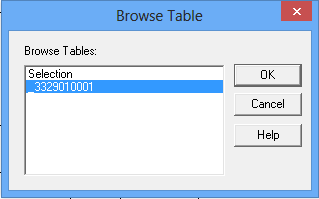
\includegraphics[width=1\textwidth]{./resources/065-jendela-browse-tabel}
    \caption{Jendela Browse Table}
  \end{figure}
  
  \item Memilih tabel mana yang hendak dibuka, dalam contoh kali ini, kita coba untuk membuka tabel milik layer 3329010001, ketika tekan tombol OK maka akan muncul jendela seperti ini :
  
  \begin{figure}[H]
    \centering
    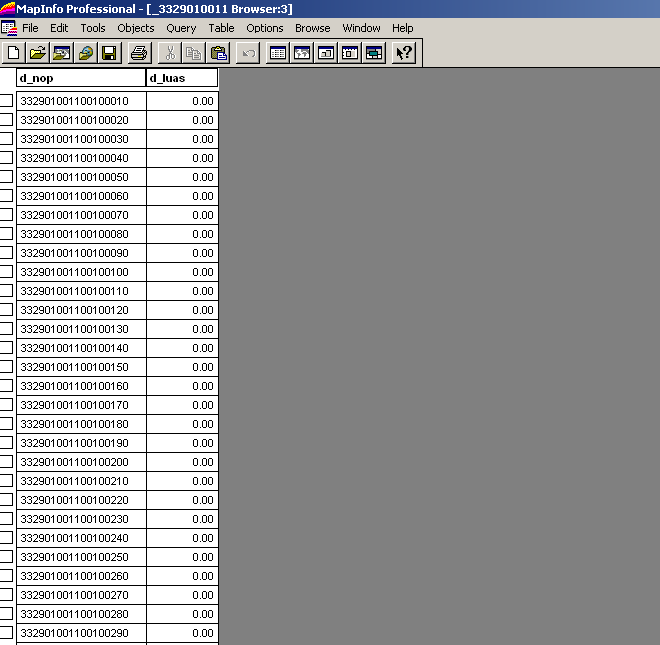
\includegraphics[width=1\textwidth]{./resources/066-isi-tabel-bidang}
    \caption{Isi Tabel Layer Bidang Objek Pajak}
  \end{figure}
\end{enumerate}

Jika melihat isi dari tabel ini, biasanya data pada \textit{field} d\_luas belum muncul, bagaimana cara memunculkannya dapat mengikuti langkah berikut :

\begin{enumerate}[1.]
  \item Pilih menu Table -\textgreater Update Column sehingga nantinya muncul jendela berikut :
  
  \begin{figure}[H]
    \centering
    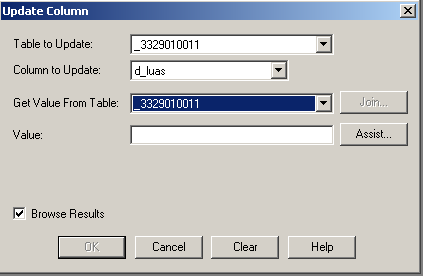
\includegraphics[width=1\textwidth]{./resources/067-jendela-update-column}
    \caption{Jendela Update Kolom}
  \end{figure}
  
  \item Biasanya perhatikan isian \textbf{Column to Update}, kolom ini yang nantinya akan kita ubah isinya, untuk selanjutnya, tekan tombol \textbf{Assist...} sehingga muncul jendela berikut :
  
  \begin{figure}[H]
    \centering
    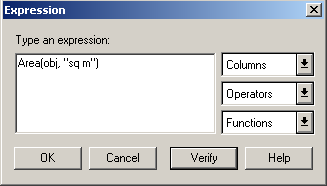
\includegraphics[width=1\textwidth]{./resources/068-jendela-expression-untuk-d_luas}
    \caption{Jendela Expression Untuk Mengisi d\_luas}
  \end{figure}
  
  \item Isikan persis seperti gambar tersebut, dan perhatikan bahwa satuan yang digunakan adalah \textbf{"sq m"} atau meter persegi. Cobalah tekan tombol \textbf{Verify} sampai dinyatakan \textit{Syntax is correct}, lalu tekan tombol \textbf{OK} sehingga tabel terisi dengan angka luasan masing-masing bidang seperti gambar berikut :
  
  \begin{figure}[H]
    \centering
    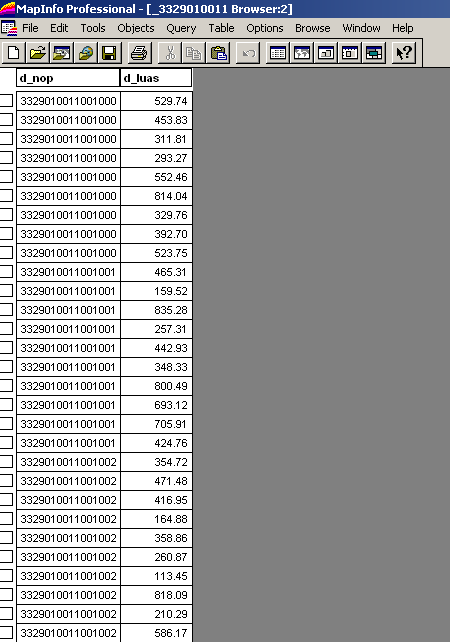
\includegraphics[width=1\textwidth]{./resources/069-hasil-update-column}
    \caption{Hasil Perhitungan Luas Bidang}
  \end{figure}
\end{enumerate}

Sekarang kita coba untuk operasi yang lebih spesifik ke \textit{query}, kita akan memilih berdasarkan blok tertentu (misal kita akan memilih blok 2), berikut adalah langkah-langkahnya :

\begin{enumerate}[1.]
  \item Memilih menu Query -\textgreater Select sehingga muncul jendela Select berikut :
  
  \begin{figure}[H]
    \centering
    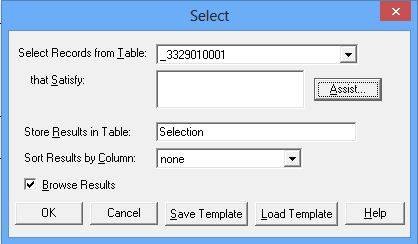
\includegraphics[width=1\textwidth]{./resources/070-jendela-select}
    \caption{Jendela Select}
  \end{figure}
  
  \item Pada bagian \textit{that satisfy}, tekan tombol \textbf{Assist} untuk mempermudah penggunaan operator dan verifikasi kode, sehingga nantinya akan muncul jendela Assist berikut :
  
  \begin{figure}[H]
    \centering
    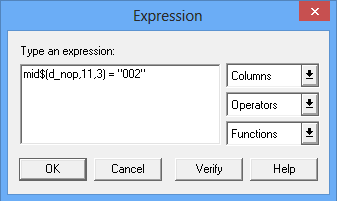
\includegraphics[width=1\textwidth]{./resources/071-jendela-expression}
    \caption{Jendela Expression}
  \end{figure}
  
  \item Isikan dengan kode berikut :
  
  \begin{lstlisting}
    mid$(d_nop,11,3)="002"
  \end{lstlisting}
  
  Jangan lupa untuk melakukan verifikasi kode setelahnya.
  
  \item Setelah menekan tombol \textbf{OK}, maka akan kembali lagi ke jendela Select, tekan \textbf{OK} kembali untuk menampilkan hasilnya yang disajikan dalam bentuk tabel. Berikut hasilnya :
  
  \begin{figure}[H]
    \centering
    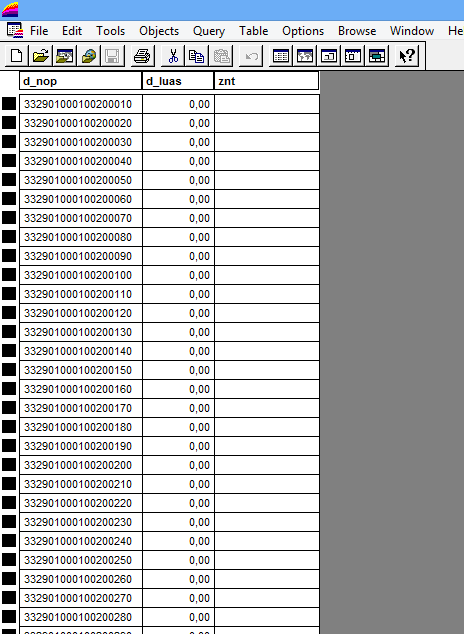
\includegraphics[width=1\textwidth]{./resources/072-hasil-select}
    \caption{Tabel Hasil Select}
  \end{figure}
  
  \item Untuk mengetahui letaknya di peta, aktifkan dahulu petanya dalam contoh ini dengan memilih menu Window -\textgreater 1. \_3329010001 Map, kemudian pilih menu Query -\textgreater Find Selection -\textgreater In Current Map Window, atau tekan Ctrl+G. Objek terpilih nantinya akan terarsir seperti gambar berikut :
  
  \begin{figure}[H]
    \centering
    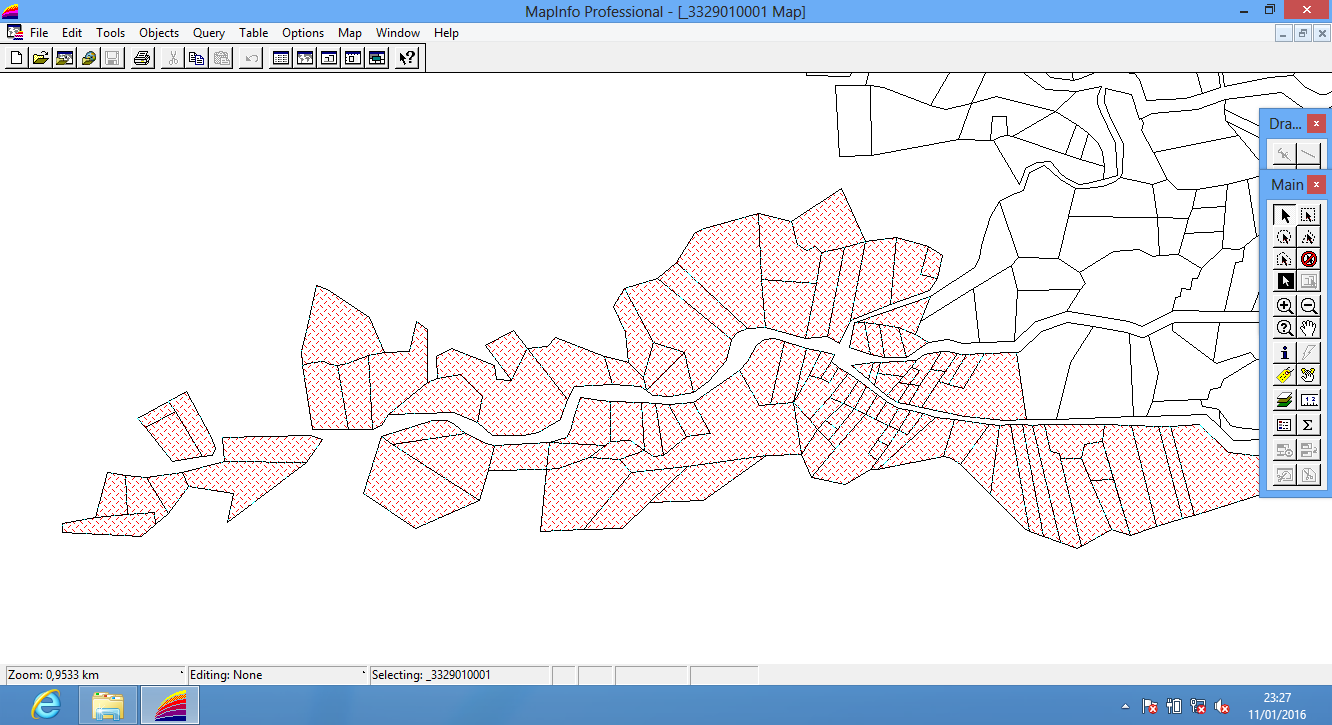
\includegraphics[width=1\textwidth]{./resources/073-hasil-pencarian-blok}
    \caption{Blok Terpilih Ditandai Dengan Bidang Terarsir}
  \end{figure}
\end{enumerate}